\section{Requerimientos}
\label{h_requerimientos}

\section{Ideas de implementaci\'on}
\label{h_ideas}

\subsection{Locomoci\'on}
\label{h_ideas_locomocion}

distintos tipos de locomocion que tuvimos en cuenta y porque elegimos este

\subsection{Sensado del entorno}
\label{h_ideas_sensado}

distintos tipos de sensores disponibles y porque elegimos estos

\subsection{Controlador}
\label{h_ideas_controlador}

distintas formas de diagramar la forma de control, que tipo de controladores necesitamos, en cuales pensamos, con cuales nos quedamos

\subsection{M\'etodo de recolecci\'on}
\label{h_ideas_recoleccion}

distintos metodos que se nos ocurrieron

\section{Actuadores}
\label{h_actuadores}

En nuestro caso, los motores son la principal forma en que el robot puede interactuar activamente con el ambiente que lo rodea.
Cada una de las tareas que deb\'iamos realizar requer\'ia de actuadores acordes.

Estas cuestiones son las que analizamos en este apartado.

\subsection{Motores de cont\'inua}
\label{h_actuadores_motorDC}

Para la tracci\'on principal de las ruedas necesitabamos motores que tuvieran el torque necesario para mover el robot, pero que pudieramos medir y
controlar la velocidad era la principal necesidad. Para esta tarea utilizamos motores de cont\'inua con caja reductora y encoder.
Con dos de estos estos motores logramos poder garantizar una velocidad determinada en las ruedas, controlar de la cantidad de movimiento en forma
independiente en cada rueda y conocer la cantidad de las vueltas dadas por cada una de las ruedas entre otras cosas.

\subsubsection{Caracter\'isticas}
\label{h_actuadores_motorDC_caracteristicas}

Los motores que elegimos son de la marca Ignis \footnote{http://www.ignis.com.ar} modelo \emph{MR-2FA} con caracter\'isticas expresadas en la tabla
\ref{hT_motorDC}, est\'an provistos de una caja reductora, poseen un encoder de $4$ estados por vuelta en el eje del motor y un sensor de de efecto
de campo para determinar una vuelta en la salida de la caja reductora.

La caja reductora provee una relaci\'on de $94$ vueltas del motor por cada $1$ vuelta del eje de salida de la caja.

En la figura \ref{hF_motorDC} mostramos las dimensiones exteriores del motor.

\begin{table}
	\begin{center}
		\begin{tabular}{|l|c|c|c|c|}
			\hline
			Caracter\'istica & Unidad & M\'inimo & Nominal & M\'aximo \\
			\hline
			Tensi\'on & V & 8 & 9 & 12 \\
			Corriente & A & 0.6 & 1.2 & 2.4 \\
			Velocidad & RPM & 1 & 60 & 60 \\
			Aceleraci\'on & $1/s^{2}$ & 0.1 & 0.1 & 0.5 \\
			Torque & kgf*cm & 0 & 1.2 & 6.4 \\
			\hline
		\end{tabular}
	\end{center}
	\caption{Caracter\'isticas del motor Ignis MR-2FA.}
	\label{hT_motorDC}
\end{table}

\begin{figure}[ht]
	\centering
	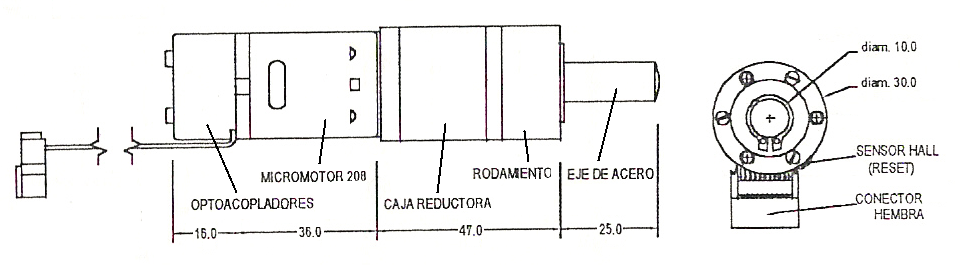
\includegraphics[scale=1]{MR2-FA.png}
	\caption{Vista lateral y frontal del motor Ignis MR-2FA. Escala $1:2$.}
	\label{hF_motorDC}
\end{figure}

Una ventaja que encontramos en este modelo es que ya trae el encoder integrado aunque su resoluci\'on podr\'ia haber sido mayor.
Los encoders los explicamos m\'as en detalle en la secci\'on \ref{h_sensado_encoder}.

\subsubsection{Circuito de control}
\label{h_actuadores_motorDC_circuito}

Para alimentar y poder controlar los motores elegimos el driver \emph{L298} de la marca ST \footnote{http://www.st.com}.
Internamente tiene dos puentes H puenteables y puede soportar hasta $4 A$. Ideal para estos motores u otros que se elijan en el futuro.

La principal funci\'on del driver era proveer de la corriente y voltaje necesarios para el funcionamiento del motor, pero la configuraci\'on
del puente H nos dio la posibilidad de, con una l\'ogica simple, determinar el sentido de la corriente y potencia que recib\'ia el motor.

Este integrado admite el puenteo de la salida aumentando as\'i la corriente que pueda circular por \'el.
Para hacer esto, conectamos las salidas \emph{Out1} y \emph{Out4} por un lado y por el otro las salidas \emph{Out2} y \emph{Out3}.
De igual forma los pines de habilitaci\'on \emph{EnA} y \emph{EnB}, luego la entrada \emph{In1} con la \emph{In4} por un lado y
por el otro la \emph{In2} con la \emph{In3}.

\begin{figure}[ht]
	\centering
	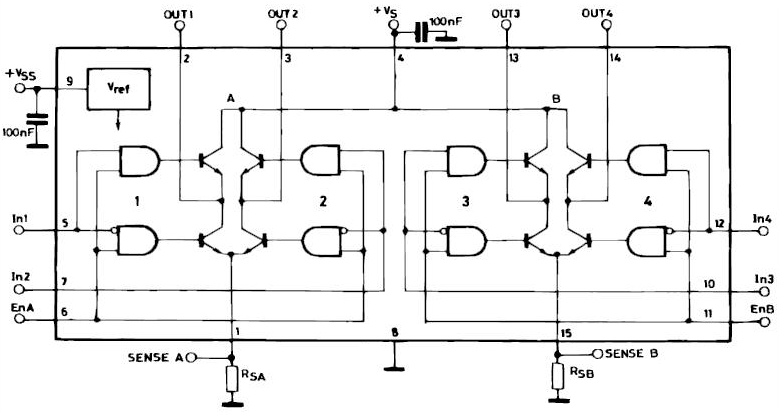
\includegraphics[scale=0.40]{L298.png}
	\caption{Diagrama interno del driver L298.}
	\label{hF_l298}
\end{figure}

De esta forma, se controla con s\'olo $3$ cables, uno de habilitaci\'on y otros $2$ de \emph{Input} que determinan
la polarizaci\'on de los transistores internos y por ende, el sentido de giro del motor.
En la tabla \ref{hT_l298} mostramos la tabla de verdad para los pines de control.
En la figura \ref{hF_l298} mostramos el diagrama interno del integrado.

\begin{table}
	\begin{center}
		\begin{tabular}{|c|c|c|c|}
			\hline
			Enable & Input $1$ & Input $2$ & Funci\'on \\
			\hline
			H & H & L & Sentido horario \\
			H & L & H & Sentido anti-horario \\
			H & L & L & Motor frenado \\
			H & H & H & Motor frenado \\
			L & X & X & Motor libre \\
			\hline
		\end{tabular}
	\end{center}
	\caption{Tabla de verdad para el control del driver \emph{L298}. Donde H es estado algo, L estado bajo y X cualquier estado.}
	\label{hT_l298}
\end{table}

Para determinar la potencia que recibir\'ia el motor usamos el m\'odulo de \emph{PWM} del microcontrolador, que explicamos m\'as en detalle en la
secci\'on \ref{h_controlador_micro_modulos}.
Variando el ancho del pulso sobre el pin de habilitaci\'on del driver determinamos la cantidad de tiempo que el motor recibe tensi\'on, lo cual
se traduce en la potencia que este tiene para realizar el movimiento.
Cuanto mayor es el tiempo en estado alto del pulso, mayor la potencia.

Para contrarrestar la corriente negativa en las salidas del driver usamos los diodos \emph{FR304} que cumplen con las especificaciones del driver
con $150$ns de tiempo de recuperaci\'on y una corriente de $3 A$.

El consumo del motor lo medimos mediante el pin de sensado en el driver, conectado a masa por una resistencia y al m\'odulo de \emph{ADC} del
microcontrolador, que explicamos en la secci\'on \ref{h_controlador_micro_modulos}.
Conociendo el valor de la resistencia y el valor leido por el m\'odulo de \emph{ADC}, pudimos determinar cuanta corriente que circulaba por la
resistencia y por ende la corriente consumida por el motor.

Para controlar la velocidad del motor usamos 1 de los 2 encoders que trae.
Conectados como entrada para el m\'odulo de \emph{Timer} del microcontrolador, en configuraci\'on de contador, que explicamos m\'as en detalle en la
secci\'on \ref{h_controlador_micro_modulos}.
Usando otro \emph{Timer} para tener una base de tiempo fija y con el valor del contador pudimos determinar y controlar la velocidad de las ruedas.

En la secci\'on \ref{h_placas_motorDC} explicamos el desarrollo de la placa controladora de estos motores.

\subsubsection{Rutinas de control}
\label{h_actuadores_motorDC_rutinas}

Desde el punto de vista del c\'odigo, tuvimos que desarrollar las rutinas necesarias para el manejo de los motores seg\'un las intrucciones del
controlador principal.

Configuramos a uno de los timers internos del microcontrolador para que genere una interrupci\'on cada $6.25$ms, la cual usamos para realizar
chequeos y ejercer control sobre el motor.
Verificamos el consumo del motor para evitar sobrecargar el circuito y los motores ante un posible atasco de las ruedas.
Tambi\'en actualizamos el acumulado de vueltas realizadas por el motor para la odometr\'ia.

Cada $200$ms, o sea $32$ interrupciones, tomamos la cantidad de cuentas del encoder, correjimos la velocidad de giro del motor ajustando el
ancho del pulso generado por el PWM.
Luego borramos el contador y esperamos otros $200$ms.

\subsection{Servo motores}
\label{h_actuadores_servo}

Para el movimiento de las partes del m\'odulo de recolecci\'on. una c\'amara con paneo y giro o un senor de ultrasonido colocado
en la parte superior haciendo las veces de radar, pensamos en el uso de servo motores.
La principal caracter\'istica de estos actuadores es que nosotros s\'olo debemos indicar el \'angulo al que queremos que este
el eje del motor y este se coloca autom\'aticamente.
El \'angulo de trabajo va desde $0^{\circ}$ a $180^{\circ}$ y algunos llegan hasta los $200^{\circ}$.

Aunque no fue implementado el ning\'un mecanismo que requiriera el uso de estos motores, explicamos en este apartado el trabajo realizado
en torno a este tipo de actuadores.
En la secci\'on \ref{h_placas_servos} explicamos el dise\~no de las placas que los controlan.

El servo de prueba que utilizamos para el desarrollo es el modelo \emph{HX5010} de la marca Hextronik \footnote{www.hextronik.com/}
con caracteristicas que expresamos en la tabla \ref{hT_hx5010}

\begin{table}
	\begin{center}
		\begin{tabular}{|c|c|c|}
			\hline
			Caracter\'istica & Unidad & Valor \\
			\hline
			Torque & kg & $6.5$ \\
			Velocidad & segundos/grado & $\frac{0.16}{60}$ \\
			Voltaje & V & $4.8$ a $6$ \\
			Delay m\'aximo & $\mu s$ & $4$ \\
			Dimensiones & $mm$ & 40x20x38 \\
			Peso & $g$ & $39$ \\
			\hline
		\end{tabular}
	\end{center}
	\caption{Caracter\'isticas del servo HX5010.}
	\label{hT_hx5010}
\end{table}

\subsubsection{Circuito de control}
\label{h_actuadores_servo_circuito}

La alimentaci\'on y consumo depende del modelo espec\'ifico, variando tambi\'en el torque que posee el servo.

No es necesario el uso de un driver para manejarlos, simplemente con la alimentaci\'on y una se\~nal con el \'angulo es suficiente.
La forma de comunicar el \'angulo var\'ia entre los distintos servos y fabricantes.
Hay servos anal\'ogicos y servos digitales.
En los primeros la posici\'on se determina mediante un voltaje que varia seg\'un cierto rango y si es digital, se setea mediante el ancho de
un pulso que tiene un tiempo m\'inimo y m\'aximo para mapear los \'angulos m\'inimo y m\'aximo respectivamente.

Dentro del modo de uso, podemos hacer que queden sueltos o que se queden fijos en cierta posici\'on indicando, de forma cont\'inua, el valor
del \'angulo requerido.
La frecuencia a la que se debe setear la posici\'on depende el modelo.

\subsubsection{Rutinas de control}
\label{h_actuadores_servo_rutinas}

Debido a que pensamos usar motores digitales y por lo menos \'ibamos a necesitar $3$ servos, necesitabamos contar con varios m\'odulos de PWM.
Como s\'olo dispon\'iamos de 1, decidimos realizar la misma funci\'on pero por software.

Usamos el timer de $16$bits del microcontrolador configurado con el clock interno de $20$MHz como medida del tiempo para crear $5$ salidas con
pulsos que var\'ian el ancho en forma independiente cada una.
Definimos un ancho m\'inimo y m\'aximo, pudiendo configurar pasos intermedios de $1^{\circ}$ (aproximadamente $69.4\mu s$).

\section{Sensado}
\label{h_sensado}

tipos de sensores elegidos y por que los elegimos

\subsection{Tel\'emetros infrarrojos}
\label{h_sensado_telemetros}

principio de funcionamiento

\subsubsection{Caracter\'isticas}
\label{h_sensado_telemetros_caracteristicas}

modelo, marca, medidas, alimentacion, consumo, tiempo de muestreo, tipo de salida, rangos de distancia, rangos de voltaje, distancia vs voltaje

\subsubsection{Circuito de control}
\label{h_sensado_telemetros_circuito}

alimentacion, conmutacion (transistor, estado de habilitacion: 0), conexion con el micro, salida del sensor, modulo ADC, muestreo, capacitor para alimentacion, circuito minimo (diagrama)

\subsubsection{Diagrama de conexi\'on}
\label{h_sensado_telemetros_diagrama}

asignacion de pines

\subsubsection{Rutinas de control}
\label{h_sensado_telemetros_rutinas}

codigo de lectura de distancia (explicacion)

\subsection{Sensor de distancia por ultrasonido}
\label{h_sensado_ultrasonido}

principio de funcionamiento

\subsubsection{Caracter\'isticas}
\label{h_sensado_ultrasonido_caracteristicas}

modelo, marca, medidas, alimentacion, consumo, tiempo/frecuencia de muestreo, tipo de salida, rangos de distancia, rango de ancho de pulso, distancia vs ancho del pulso

\subsubsection{Circuito de control}
\label{h_sensado_ultrasonido_circuito}

alimentacion, conmutacion (transistor, estado de habilitacion: 0), conexion con el micro, salida del sensor, modulo ADC, muestreo, capacitor para alimentacion, circuito minimo (diagrama)

\subsubsection{Diagrama de conexi\'on}
\label{h_sensado_ultrasonido_diagrama}

asignacion de pines

\subsubsection{Rutinas de control}
\label{h_sensado_ultrasonido_rutinas}

codigo de lectura de distancia (explicacion)

\subsection{Sensor reflectivo de piso}
\label{h_sensado_piso}

principio de funcionamiento

\subsubsection{Caracter\'isticas}
\label{h_sensado_piso_caracteristicas}

modelo, marca, medidas, alimentacion, consumo, tiempo/frecuencia de muestreo, tipo de salida, distancia optima, rangos de voltaje, distancia vs voltaje

\subsubsection{Circuito de control}
\label{h_sensado_piso_circuito}

alimentacion, resistencias elegidas, conmutacion (transistor, estado de habilitacion: 0), conexion con el micro, salida del sensor, modulo ADC, muestreo, capacitor para alimentacion, circuito minimo (diagrama)

\subsubsection{Diagrama de conexi\'on}
\label{h_sensado_piso_diagrama}

asignacion de pines

\subsubsection{Rutinas de control}
\label{h_sensado_piso_rutinas}

codigo de lectura de nivel de reflexion (explicacion)

\subsection{Encoders}
\label{h_sensado_encoder}

principio de funcionamiento

estamos usando solo uno de los sensores del encoder

\subsubsection{Caracter\'isticas}
\label{h_sensado_encoder_caracteristicas}

tipo de encoders, cuentas x vuelta de eje de motor, velocidad maxima y minima recomendable

relacion de caja 94:1
max recomendable: 300 cuentas x segundo
min recomendable: 60 - 70 cuentas x segundo

\subsubsection{Circuito de control}
\label{h_sensado_encoder_circuito}

alimentacion, conexionado, circuito, resistencias pull-up, swtch selector, timer/counter

\subsubsection{Diagrama de conexi\'on}
\label{h_sensado_encoder_diagrama}

asignacion de pines

\subsubsection{Rutinas de control}
\label{h_sensado_encoder_rutinas}

codigo de lectura y correcion de la velocidad del motor (explicacion)

\subsection{Sensado de la bateria}
\label{h_sensado_bateria}

principio de funcionamiento

\subsubsection{Caracter\'isticas}
\label{h_sensado_bateria_caracteristicas}

grafico/tabla de voltaje bateria vs salida

\subsubsection{Circuito de control}
\label{h_sensado_bateria_circuito}

conexionado, circuito, modulo ADC, muestreo

\subsubsection{Rutinas de control}
\label{h_sensado_bateria_rutina}

codigo de lectura de nivel de tension en la bateria (explicacion)

\subsection{Consumo del motor}
\label{h_sensado_consumo}

principio de funcionamiento

\subsubsection{Caracter\'isticas}
\label{h_sensado_consumo_caracteristicas}

grafico/tabla de corriente consumida vs voltaje, caracteristicas del puente H, valores maximos y minimos, mensajes de consumo alto

\subsubsection{Circuito de control}
\label{h_sensado_consumo_circuito}

valor de la resistencia, circuito, modulo ADC, muestreo, vref en el micro

\subsubsection{Rutinas de control}
\label{h_sensado_consumo_rutinas}

codigo de lectura de nivel de tension en la bateria (explicacion)

\subsubsection{Pulsador u otro dispositivo disparador}
\label{h_sensado_pulsador}

posibilidad de poner un pulsador o cualquier otro dispositivo que genere un cambio de estado y lo detecte como trigger

\subsubsection{Caracter\'isticas}
\label{h_sensado_pulsador_caracteristicas}

como deberia ser el boton o algun otro dispositivo que vayamos a poner ahi

\subsubsection{Circuito de control}
\label{h_sensado_pulsador_circuito}

alimentacion, consumo, circuito, interrupciones

\subsubsection{Rutinas de control}
\label{h_sensado_pulsador_rutinas}

codigo de lectura de cambio de estado en el pin de trigger (explicacion)

\section{Controladores}
\label{h_controlador}

\subsection{Netbook}
\label{h_controlador_netbook}

modelo, marca, caracteristicas, para que se usa, sistema operativo y lenguaje de programacion

\subsection{Microcontrolador}
\label{h_controlador_micro}

para que vamos a usar el micro y sus funciones principales

\subsubsection{Caracter\'isticas}
\label{h_controlador_micro_caracteristicas}

modelo, marca, familia, memorias, etc

\subsubsection{Diagrama del microcontrolador}
\label{h_controlador_micro_diagrama}

grafico y asignacion de pines x modulo

\subsubsection{M\'odulos internos}
\label{h_controlador_micro_modulos}

listado de modulos que tiene y caracteristicas de cada uno

\subsubsection{Programaci\'on del firmware}
\label{h_controlador_micro_programacion}

pines de programacion, icd2, IDE, lenguaje, version

\section{Comunicaci\'on}
\label{h_comm}

porque necesitamos comunicar los modulos, que necesidades hay, nivel de uso

\subsection{Conectividad entre m\'odulos}
\label{h_comm_conectividad}

daisy chain, diagrama, montado sobre rs232, control de errores

\subsection{Protocolo de comunicaci\'on}
\label{h_comm_protocolo}

caracteristicas necesarias en el protocolo, porque es importante, cosas que tuvimos en cuenta y decisiones, control de errores

\subsubsection{Caracter\'isticas b\'asicas}
\label{h_comm_protocolo_caracteristicas}

formado por paquetes, formato basico del paquete (header), control de errores

\subsubsection{Comandos comunes}
\label{h_comm_protocolo_comandosComunes}

contelo o listado de comandos comunes (en detalle o se van a un apendice) - son pocos.

\subsubsection{Comandos espec\'ificos}
\label{h_comm_protocolo_comandosEspecificos}

contelo o listado de comandos especificos segun el tipo de placa (referencia a un apendice con cada uno explicado)

\subsubsection{Estad\'isticas}
\label{h_comm_protocolo_estadisticas}

analisis de paquetes por segundo, bytes de datos vs bytes de header, retransmisiones, etc

\section{Placas controladoras}
\label{h_placas}

porque tuvimos que diseñar nuestras propias placas, cosas que tuvimos en cuenta y decisiones tomadas, codigos fuente a los apendices

\subsection{Placa gen\'erica}
\label{h_placas_generica}

funcion de una placa generica, porque fue armada, para que sirve

\subsubsection{Caracter\'isticas principales}
\label{h_placas_generica_caracteristicas}

testeo de nuevos modulos, testeo de la programacion, snifear la comunicacion, futuras expansiones

\subsubsection{M\'odulo de comunicaci\'on}
\label{h_placas_generica_comm}

explicacion de la comunicacion, igual en todas, switch de configuracion, pines, fichas, nodos en la cadena, cables pc-placa y placa-placa, max232

\subsubsection{Alimentaci\'on de la placa}
\label{h_placas_generica_alimentacion}

tension para la alimentacion, circuito de la fuente, consumo maximo, voltaje minimo de alimentacion, alimentacion de 5V directos

\subsubsection{Configuraci\'on}
\label{h_placas_generica_config}

configuracion minima de la placa, leds, comunicacion, header de programacion

\subsubsection{Esquem\'atico}
\label{h_placas_generica_esquematicos}

esquematicos de la placa

\subsubsection{Circuito}
\label{h_placas_generica_circuito}

circuito de la placa

\subsubsection{C\'odigo b\'asico}
\label{h_placas_generica_codigo}

explicacion de lo minimo que deberia tener para ser parte de la cadena de comunicacion

\subsubsection{Posibles extensiones}
\label{h_placas_generica_extensiones}

posibles extensiones a futuro de la placa - nuevos modulos de testeo o control o lectura muy basica de señales, pasar a montaje superficial los componentes, hacerla mas chica

\subsection{Placa controladora de motores DC}
\label{h_placas_motorDC}

funcion de una placa controladora de motorDC, porque fue armada, para que sirve, porque hay 2, porque no esta en una sola

\subsubsection{Caracter\'isticas principales}
\label{h_placas_motorDC_caracteristicas}

principio de funcionamiento, como logra controlar la velocidad, como logra ser parte de la cadena, como logra sensar el consumo, controlar el motor, puente H, diodos, leds, VREF

\subsubsection{M\'odulo de comunicaci\'on}
\label{h_placas_motorDC_comm}

se explico en el modulo generico, se agregan los comandos especificos y se puede explicar como se obtiene la informacion para dar las respuestas

\subsubsection{Alimentaci\'on de la placa}
\label{h_placas_motorDC_alimentacion}

se explico en el modulo generico, tension para la alimentacion para los motores, necesidad de masa unica como referencia, consumo aproximado de los motores

\subsubsection{Configuraci\'on}
\label{h_placas_motorDC_config}

configuracion de la placa, leds, comunicacion, header de programacion, switch de seleccion de encoder

\subsubsection{Esquem\'atico}
\label{h_placas_motorDC_esquematico}

esquematicos de la placa

\subsubsection{Circuito}
\label{h_placas_motorDC_circuito}

circuito de la placa

\subsubsection{C\'odigo b\'asico}
\label{h_placas_motorDC_codigo}

explicacion de lo minimo que deberia tener para ser parte de la cadena de comunicacion, sensado y control de la velocidad de los motores

\subsubsection{Posibles extensiones}
\label{h_placas_motorDC_extensiones}

unificar en una placa el control de mas de un motor, pasar a montaje superficial los componentes, hacerla mas chica

\subsection{Placas de sensado}
\label{h_placas_sensado}

funcion de una placa de sensado, porque fue armada, para que sirve, que tipo de sensores puedo conectar, cuales son las posibles configuraciones, diferencias, sensado de la bateria

\subsubsection{Caracter\'isticas principales}
\label{h_placas_sensado_caracteristicas}

principio de funcionamiento, como logra tomar las muestras de los sensores, como logra ser parte de la cadena, seteo de los tipos de sensores

\subsubsection{M\'odulo de comunicaci\'on}
\label{h_placas_sensado_comm}

se explico en el modulo generico, se agregan los comandos especificos y se puede explicar como se obtiene la informacion para dar las respuestas

\subsubsection{Alimentaci\'on de la placa}
\label{h_placas_sensado_alimentacion}

se explico en el modulo generico

\subsubsection{Configuraci\'on}
\label{h_placas_sensado_config}

configuracion de la placa, comunicacion, header de programacion

\subsubsection{Esquem\'atico}
\label{h_placas_sensado_esquematico}

esquematicos de la placa

\subsubsection{Circuito}
\label{h_placas_sensado_circuito}

circuito de la placa

\subsubsection{C\'odigo b\'asico}
\label{h_placas_sensado_codigo}

explicacion de lo minimo que deberia tener para ser parte de la cadena de comunicacion y sensado de los distintos perifericos

\subsubsection{Posibles extensiones}
\label{h_placas_sensado_extensiones}

uso de componentes como resistencias variables para regular la alimentacion de los sensores de piso y resistencias pull-up, pasar a montaje superficial los componentes, hacerla mas chica

\subsection{Placa controladora de servo motores}
\label{h_placas_servos}

funcion de una placa controladora de servos, porque no fue armada, para que se penso, alguna otra opcion de conexion, pines libres

\subsubsection{Caracter\'isticas principales}
\label{h_placas_servos_caracteristicas}

principio de funcionamiento, como logra generar varios pwm por software, como logra ser parte de la cadena

\subsubsection{M\'odulo de comunicaci\'on}
\label{h_placas_servos_comm}

se explico en el modulo generico, se agregan los comandos especificos y se puede explicar como se obtiene la informacion para dar las respuestas

\subsubsection{Alimentaci\'on de la placa}
\label{h_placas_servos_alimentacion}

se explico en el modulo generico, con modificaciones que permiten que circule una mayor cantidad de corriente para alimentar a los servos.

\subsubsection{Configuraci\'on}
\label{h_placas_servos_config}

configuracion de la placa, comunicacion, header de programacion

\subsubsection{Esquem\'atico}
\label{h_placas_servos_esquematico}

esquematicos de la placa

\subsubsection{Circuito}
\label{h_placas_servos_circuito}

circuito de la placa

\subsubsection{C\'odigo b\'asico}
\label{h_placas_servos_codigo}

explicacion de lo minimo que deberia tener para ser parte de la cadena de comunicacion y control de los servos

\subsubsection{Posibles extensiones}
\label{h_placas_servos_extensiones}

uso de componentes como resistencias variables para regular la alimentacion de los sensores de piso y resistencias pull-up, pasar a montaje superficial los componentes, hacerla mas chica

\section{Armado del prototipo}
\label{h_prototipo}

\subsection{Dise\~no}
\label{h_prototipo_diseno}

\subsection{Caracter\'isticas}
\label{h_prototipo_caracteristicas}

con las ruedas de 10cm y teniendo en cuenta que el motor gira a unas 300 cuentas/segundo (usando un solo sensor en el encoder) llegamos a 50 cm/s de velocidad

\subsection{Desarme}
\label{h_prototipo_desarme}

\subsection{Costo y proveedores}
\label{h_prototipo_costo}
